\documentclass[12pt]{article}
\usepackage[english]{babel}
\usepackage[utf8]{inputenc}

%% Pointer to 'default' preamble
% pacakages and definitions

\usepackage{geometry}
\geometry{
	letterpaper, 
	portrait, 
	top=.75in,
	left=.8in,
	right=.75in,
	bottom=.5in		} 	% Page Margins
	
%% additional packages for nice things
\usepackage{amsmath} 	% for most math
\usepackage{commath} 	% for abs
\usepackage{lastpage}	% for page count
\usepackage{amssymb} 	% for therefore
\usepackage{graphicx} 	% for image handling
\usepackage{wrapfig} 	% wrap figures
\usepackage[none]{hyphenat} % for no hyphenations
\usepackage{array} 		% for >{} column characterisctis
\usepackage{physics} 	% for easier derivative \dv....
\usepackage{tikz} 		% for graphic@!
\usepackage{circuitikz} % for circuits!
\usetikzlibrary{arrows.meta} % for loads
\usepackage[thicklines]{cancel}	% for cancels
\usepackage{xcolor}		% for color cancels
\usepackage[per-mode=fraction]{siunitx} % for si units and num
\sisetup{group-separator = {,}, group-minimum-digits = 3} % additional si unit table functionality

\usepackage{fancyhdr} 	% for header
\usepackage{comment}	% for ability to comment out large sections
\usepackage{multicol}	% for multiple columns using multicols
\usepackage[framed,numbered]{matlab-prettifier} % matlab sytle listing
\usepackage{marvosym} 	% for boltsymbol lightning
\usepackage{pdflscape} 	% for various landscape pages in portrait docs.
%\usepackage{float}
\usepackage{fancyvrb}	% for Verbatim (a tab respecting verbatim)
\usepackage{enumitem}	% for [resume] functionality of enumerate
\usepackage{spreadtab} 	% for using formulas in tables}
\usepackage{numprint}	% for number format in spread tab
\usepackage{subcaption} % for subfigures with captions
\usepackage[normalem]{ulem} % for strike through sout

% for row colors in tables....
\usepackage{color, colortbl}
\definecolor{G1}{gray}{0.9}
\definecolor{G2}{rgb}{1,0.88,1}%{gray}{0.6}
\definecolor{G3}{rgb}{0.88,1,1}

% For table formatting
\usepackage{booktabs}
\renewcommand{\arraystretch}{1.2}
\usepackage{floatrow}
\floatsetup[table]{capposition=top} % put table captions on top of tables

% Caption formating footnotesize ~ 10 pt in a 12 pt document
\usepackage[font={small}]{caption}

%% package config 
\sisetup{output-exponent-marker=\ensuremath{\mathrm{E}}} % for engineer E
\renewcommand{\CancelColor}{\color{red}}	% for color cancels
\lstset{aboveskip=2pt,belowskip=2pt} % for more compact table
%\arraycolsep=1.4pt\def
\setlength{\parindent}{0cm} % Remove indentation from paragraphs
\setlength{\columnsep}{0.5cm}
\lstset{
	style      = Matlab-editor,
	basicstyle = \ttfamily\footnotesize, % if you want to use Courier - not really used?
}
\renewcommand*{\pd}[3][]{\ensuremath{\dfrac{\partial^{#1} #2}{\partial #3}}} % for larger pd fracs
\renewcommand{\real}[1]{\mathbb{R}\left\{ #1 \right\}}	% for REAL symbol
\newcommand{\imag}[1]{\mathbb{I}\left\{ #1 \right\}}	% for IMAG symbol
\definecolor{m}{rgb}{1,0,1}	% for MATLAB matching magenta
	
%% custom macros
\newcommand\numberthis{\addtocounter{equation}{1}\tag{\theequation}} % for simple \numberthis command

\newcommand{\equal}{=} % so circuitikz can have an = in the labels
\newcolumntype{L}[1]{>{\raggedright\let\newline\\\arraybackslash\hspace{0pt}}m{#1}}
\newcolumntype{C}[1]{>{\centering\let\newline\\\arraybackslash\hspace{0pt}}m{#1}}
\newcolumntype{R}[1]{>{\raggedleft\let\newline\\\arraybackslash\hspace{0pt}}m{#1}}

%% Header
\pagestyle{fancy} % for header stuffs
\fancyhf{}
% spacing
\headheight 29 pt
\headsep 6 pt

%% Header
\rhead{Thad Haines \\ Page \thepage\ of \pageref{LastPage}}
\chead{Kundur Four Machine for LTD\\ Step and Ramp Comparisons}
\lhead{Research \\ }

\begin{document}
\paragraph{System Information}
\newcommand{\figW}{1}
	\begin{figure}[h!]
			\centering
			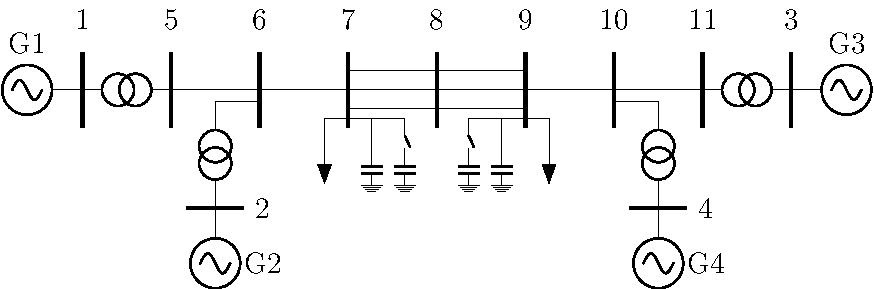
\includegraphics[width=\figW\linewidth]{kundur4LTD.pdf}\vspace{-.5em}
			\caption{Slightly Modified Kundur System.}
			\label{system}		 
	\end{figure}%\vspace{-0em}
% uses sameGens5.dyd
\begin{Verbatim}

#   generators
genrou   1 "1" 22.00 "1 " : #9 mva=600.00   ... "h" 6   "d" 0.0000 ... "ra" 0.0000 ...
genrou   2 "2" 22.00 "1 " : #9 mva=800.00   ... "h" 4   "d" 0.0000 ... "ra" 0.0000 ...
genrou   3 "3" 22.00 "1 " : #9 mva=1100.00  ... "h" 3   "d" 0.0000 ... "ra" 0.0000 ...
genrou   4 "4" 22.00 "1 " : #9 mva=900.00   ... "h" 4   "d" 0.0000 ... "ra" 0.0000 ...

#   exciters
sexs     1 "1" 22.00 "1 " : #9 1.0 5.0 1000.0 0.05 -5.0 5.0 0.1 0.0 -5.0 5.0 0.0
sexs     2 "2" 22.00 "1 " : #9 1.0 5.0 1000.0 0.05 -5.0 5.0 0.1 0.0 -5.0 5.0 0.0
sexs     3 "3" 22.00 "1 " : #9 1.0 5.0 1000.0 0.05 -5.0 5.0 0.1 0.0 -5.0 5.0 0.0
sexs     4 "4" 22.00 "1 " : #9 1.0 5.0 1000.0 0.05 -5.0 5.0 0.1 0.0 -5.0 5.0 0.0

#   governors                            R      T1           T2      T3
tgov1 1 "1" 22.00 "1 " : #1 mwcap=450.00 0.040  0.4 1.00 0.0 3.0000  10.0000 0.0
tgov1 2 "2" 22.00 "1 " : #1 mwcap=500.00 0.050  0.4 1.00 0.0 3.0000  10.0000 0.0
tgov1 3 "3" 22.00 "1 " : #1 mwcap=700.00 0.030  0.4 1.00 0.0 3.0000  10.0000 0.0

....
At t = 0:
Load on bus 7 = 400 P, 100 Q
Load on bus 9 = 500 P, 100 Q
Slack 240 Pegn 31 Qgen
All other Gens approx 220 Pgen, 26 Qgen
approx 60 MW Interchange from Area 1 to Area 2 (left to right)
\end{Verbatim}


\pagebreak
\newcommand{\caseName}{kundurStep}
\paragraph{Step Test:} Load on Bus 9 -30\% at t=2
	\begin{figure}[h!]
			\centering
			\includegraphics[width=\figW\linewidth]{\caseName F}\vspace{-.5em}
			\caption{System frequency response.}
			\label{\caseName F}		 
	\end{figure}%\vspace{-0em}
	\begin{figure}[h!]
			\centering
			\includegraphics[width=\figW\linewidth]{\caseName AveF}\vspace{-.5em}
			\caption{Average frequency.}
			\label{\caseName AveF}		 
	\end{figure}%\vspace{-0em}

	\begin{figure}[h!]
			\centering
			\includegraphics[width=\figW\linewidth]{\caseName RelF}\vspace{-.5em}
			\caption{Relative Hz difference of PSDS - LTD $\left( \text{i.e. }  \left|f_{PSDS}(t)- f_{LTD}(t)\right| \times 60 \text{Hz} \right)$.}
			\label{\caseName RelF}		 
	\end{figure}%\vspace{-.5em}
%
\pagebreak
	\begin{figure}[h!]
			\centering
			\includegraphics[width=\figW\linewidth]{\caseName Pe}\vspace{-.5em}
			\caption{Electrical Power Output}
			\label{\caseName Pe}		 
	\end{figure}%\vspace{-0em}
	\begin{figure}[h!]
			\centering
			\includegraphics[width=\figW\linewidth]{\caseName Pm}\vspace{-.5em}
			\caption{Generator Mechanical Power Output}
			\label{\caseName Pm}		 
	\end{figure}%\vspace{-0em}

\pagebreak
	\begin{figure}[h!]
			\centering
			\includegraphics[width=\figW\linewidth]{\caseName Q}\vspace{-.5em}
			\caption{Reactive Power Output}
			\label{\caseName Q}		 
	\end{figure}%\vspace{-.5em}

	\begin{figure}[h!]
			\centering
			\includegraphics[width=\figW\linewidth]{\caseName V}\vspace{-.5em}
			\caption{System Bus Voltages}
			\label{\caseName V}		 
	\end{figure}%\vspace{-0em}
	\begin{figure}[h!]
			\centering
			\includegraphics[width=\figW\linewidth]{\caseName Angle}\vspace{-.5em}
			\caption{Generator Angles}
			\label{\caseName Angle}		 
	\end{figure}%\vspace{-0em}


\pagebreak
\renewcommand{\caseName}{kundurRamp}
\renewcommand{\figW}{1}
\paragraph{Ramp Test:} Load on Bus 9 -30\% from t=2 to 42.
	\begin{figure}[h!]
			\centering
			\includegraphics[width=\figW\linewidth]{\caseName F}\vspace{-.5em}
			\caption{System frequency response.}
			\label{\caseName F}		 
	\end{figure}%\vspace{-0em}
	\begin{figure}[h!]
			\centering
			\includegraphics[width=\figW\linewidth]{\caseName AveF}\vspace{-.5em}
			\caption{Average frequency.}
			\label{\caseName AveF}		 
	\end{figure}%\vspace{-0em}


	\begin{figure}[h!]
			\centering
			\includegraphics[width=\figW\linewidth]{\caseName RelF}\vspace{-.5em}
			\caption{Relative Hz difference of PSDS - LTD $\left( \text{i.e. }  \left|f_{PSDS}(t)- f_{LTD}(t)\right| \times 60 \text{Hz} \right)$.}
			\label{\caseName RelF}		 
	\end{figure}%\vspace{-.5em}

\pagebreak
	\begin{figure}[h!]
			\centering
			\includegraphics[width=\figW\linewidth]{\caseName Pe}\vspace{-.5em}
			\caption{Electrical Power Output.}
			\label{\caseName Pe}		 
	\end{figure}%\vspace{-0em}
	\begin{figure}[h!]
			\centering
			\includegraphics[width=\figW\linewidth]{\caseName Pm}\vspace{-.5em}
			\caption{Generator Mechanical Power Output}
			\label{\caseName Pm}		 
	\end{figure}%\vspace{-0em}


\pagebreak

	\begin{figure}[h!]
			\centering
			\includegraphics[width=\figW\linewidth]{\caseName Q}\vspace{-.5em}
			\caption{Reactive Power Output}
			\label{\caseName Q}		 
	\end{figure}%\vspace{-.5em}

	\begin{figure}[h!]
			\centering
			\includegraphics[width=\figW\linewidth]{\caseName V}\vspace{-.5em}
			\caption{System Bus Voltages}
			\label{\caseName V}		 
	\end{figure}%\vspace{-0em}
	\begin{figure}[h!]
			\centering
			\includegraphics[width=\figW\linewidth]{\caseName Angle}\vspace{-.5em}
			\caption{Generator Angles}
			\label{\caseName Angle}		 
	\end{figure}%\vspace{-0em}

\end{document}